\documentclass[letterpaper,10pt,conference]{ieeeconf}

\IEEEoverridecommandlockouts
\overrideIEEEmargins

\usepackage{graphicx}
\usepackage{amsmath}
\usepackage{amssymb}
\usepackage{booktabs}
\usepackage{cite}
\usepackage{url}
\usepackage{array}

\graphicspath{{./}}

% Replace each semantic result macro only with a value exported by the frozen
% evaluator. They intentionally remain independent to prevent metric mixing.
\newcommand{\TDB}{\ensuremath{\mathbf{TDB}}}
\newcommand{\MSCAAAP}{\ensuremath{0.6306}}
\newcommand{\MSCAAAPFifty}{\ensuremath{0.9286}}
\newcommand{\MSCAAHumanAP}{\ensuremath{0.7842}}
\newcommand{\MSCAAFishAP}{\ensuremath{0.4770}}
\newcommand{\SAFusionAP}{\ensuremath{0.6245}}
\newcommand{\SAFusionAPFifty}{\ensuremath{0.9370}}
\newcommand{\SAFusionHumanAP}{\ensuremath{0.7932}}
\newcommand{\SAFusionFishAP}{\ensuremath{0.4558}}
\newcommand{\JointAP}{\ensuremath{0.6440}}
\newcommand{\JointAPFifty}{\ensuremath{0.9446}}
\newcommand{\JointHumanAP}{\ensuremath{0.7992}}
\newcommand{\JointFishAP}{\ensuremath{0.4888}}
\newcommand{\JointInteraction}{\ensuremath{0.0032}}

\title{\LARGE\bfseries
Content-Adaptive Pyramid Recalibration for Lightweight
Object Detection in Underwater Robotics}

% Anonymous initial submission; restore author information only after acceptance.
\author{Anonymous Authors}

\begin{document}
\maketitle
\thispagestyle{empty}
\pagestyle{empty}

\begin{abstract}
Lightweight underwater object detection provides visual cues for robotic perception, requiring both fine-scale target details and broader spatial context under constrained computational budgets. This letter proposes a hierarchical, content-adaptive pyramid recalibration design for StarEye that coordinates cross-source channel weighting with within-block spatial refinement. Scale-Aware Fusion (SAFusion) generates image-dependent channel weights from a joint descriptor of aligned pyramid features. Multi-Scale Context-Aware Attention (MSCAA) extends Context Anchor Attention (CAA) with two spatial context extents, using shared preprocessing and learned response fusion to generate channel-specific spatial masks. The resulting fusion-to-refinement hierarchy first recalibrates concatenated pyramid channels and then refines their transformed representations within C2f-Star blocks, while retaining the original pyramid topology and detection head. Under a common three-seed protocol, mean validation \(\mathrm{mAP}_{50:95}\) increases from \(0.6143\) to \(0.6440\), a gain of \(2.97\) percentage points. Human and fish AP improve by \(2.28\) and \(3.67\) percentage points, respectively. The model contains \(3.62\) million parameters and requires \(25.7\) GFLOPs at \(640\times640\), representing increases of \(17.9\%\) and \(4.5\%\) over StarEye. Factorial ablation shows complementary module contributions, with the joint design exceeding the stronger single-module configuration by \(1.34\) AP points.

\end{abstract}

% Candidate keywords retained for submission metadata, not typeset here:
% Underwater object detection, underwater robotics, multi-scale context,
% feature pyramid, content-adaptive fusion.

\section{Introduction}
Underwater object detection supports robotic perception
for diver monitoring and aquatic target observation~\cite{ref_duo,ref_vddc}.
Computational efficiency is important for onboard perception,
motivating compact feature extractors~\cite{ref_mobilenetv2,ref_ghostnet}.
Wavelength-dependent attenuation and backscatter reduce contrast and
obscure local structure~\cite{ref_jaffe,ref_seathru}.
Nearby swimmers and small aquatic targets may coexist, requiring both
body-scale structure and fine spatial evidence.

Existing methods either restore images before detection or adapt the
detector~\cite{ref_survey,ref_swipenet,ref_amspuod}.
Image enhancement can improve visibility without necessarily improving
detection performance~\cite{ref_uieb,ref_enhance1,ref_enhance2}.
End-to-end alternatives adapt feature or domain representations
within the detector~\cite{ref_e2e1,ref_e2e2}.
Feature pyramids combine high-resolution detail with deep
semantics~\cite{ref_fpn,ref_panet,ref_efficientdet}.
Channel attention models inter-channel dependencies, while joint
channel--spatial attention refines features along both
dimensions~\cite{ref_senet,ref_cbam}.

This letter builds on StarEye~\cite{ref_stareye}, a compact detector
combining a StarNet-S050 backbone~\cite{ref_starnet}, a CAA-enhanced
neck~\cite{ref_caa}, and an SCBN head. Two related representation challenges motivate the proposed neck design. At cross-level fusion junctions, direct concatenation preserves pyramid features but provides no explicit input-dependent channel weighting before refinement. Within C2f-Star, each CAA mask uses a single context extent, limiting the contextual evidence available to its generator. Addressing these two aspects together motivates a hierarchy in which cross-source channel recalibration precedes dual-extent spatial refinement.

We coordinate SAFusion and MSCAA in the StarEye neck: SAFusion recalibrates
concatenated pyramid features using their joint descriptor, and MSCAA refines
the resulting representations within C2f-Star. This ordering conditions
spatial refinement on cross-source channel weighting.

The main contributions are threefold. First, we introduce MSCAA, a dual-extent context modulation module that combines shared preprocessing, factorized strip convolutions, and learned response fusion to construct channel-specific spatial masks from both broader and more localized evidence. Second, we design SAFusion to recalibrate concatenated pyramid channels using a joint cross-source descriptor, enabling the weight of each source channel to depend on information from both fusion inputs. Third, we integrate the two modules into a consistent fusion-to-refinement hierarchy across all four bidirectional pyramid junctions. A three-seed factorial ablation demonstrates complementary contributions, with a \(2.97\)-point gain in overall AP at a \(4.5\%\) increase in reported FLOPs.

\section{Content-Adaptive Pyramid Recalibration}
\subsection{Overall Architecture and Design Scope}
Fig.~\ref{fig:architecture} presents the joint detector. For a \(640\times640\) input, StarNet-S050 produces feature maps \(\{\mathbf P_3,\mathbf P_4,\mathbf P_5\}\) at spatial resolutions of \(80\times80\), \(40\times40\), and \(20\times20\), respectively. The bidirectional FPN/PAN topology is retained: MSCAA replaces CAA inside C2f-Star, SAFusion augments each of the four cross-level concatenation junctions with channel recalibration, and the SCBN head retains the original three detection scales.

Let \(\mathbf{X}_{i}^{q}\) and \(\mathbf{X}_{j}^{q}\) denote the actual inputs to
junction \(q\); either may be a backbone output or an intermediate neck feature.
The alignment operator \(\mathcal{R}_{i\leftarrow j}^{q}\) is nearest-neighbor
upsampling, learned stride-two convolution, or identity. The implemented
junction is
\begin{align}
 \mathbf{F}_{i}^{q}&=
 [\,\mathcal{R}_{i\leftarrow j}^{q}(\mathbf{X}_{j}^{q});
       \mathbf{X}_{i}^{q}\,],\nonumber\\
 \mathbf{Z}_{i}^{q}&=\mathcal{S}_{i}^{q}(\mathbf{F}_{i}^{q}),\nonumber\\
 \mathbf{Y}_{i}^{q}&=\mathcal{B}_{i}^{q,\mathrm{MSCAA}}
       (\mathbf{Z}_{i}^{q}),
 \label{eq:joint_map}
\end{align}
Here, \([\cdot;\cdot]\) denotes channel concatenation, \(\mathcal S_i^q\) is the channel recalibration stage of SAFusion at junction \(q\), and \(\mathcal B_i^{q,\mathrm{MSCAA}}\) is the subsequent C2f-Star block with MSCAA embedded in each Star block.

\begin{figure*}[t]
  \centering
  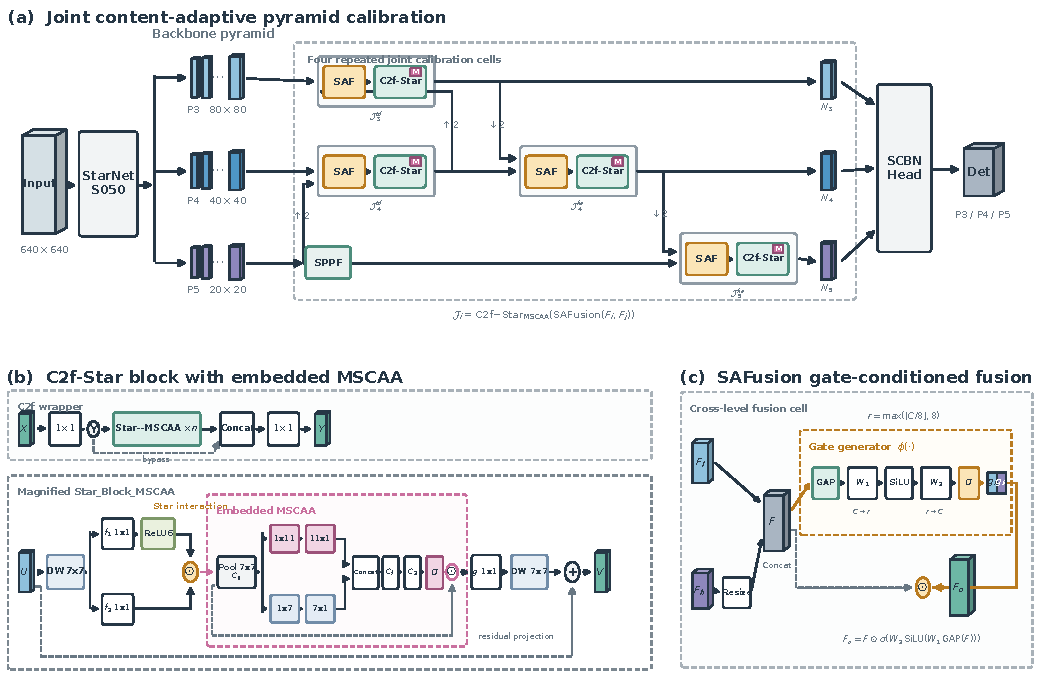
\includegraphics[width=\textwidth]{joint_mscaa_safusion_advanced}
  \caption{Joint calibration neck. (a) Four SAFusion--C2f-Star cells replace
static FPN/PAN fusion stages; perspective depth denotes channels,
not 3-D convolution.
(b) The C2f wrapper retains a partial-gradient bypass; the magnified
Star block shows multiplicative interaction, embedded dual-strip MSCAA,
projection, and residual path.
(c) SAFusion concatenates spatially aligned pyramid features and
generates an image-dependent channel gate from their joint global descriptor.}
  \label{fig:architecture}
\end{figure*}

\subsection{Dual-Extent Spatial Context Modulation}
MSCAA uses shared preprocessing to feed two parallel strip-convolution paths,
fusing their responses to generate channel-specific spatial masks from broader
and more localized context without duplicating the entire attention module.
Given
\(\mathbf{X}\in\mathbb{R}^{B\times C\times H\times W}\), MSCAA first applies the
shared local preprocessing used by CAA,
\begin{equation}
 \mathbf{U}=\mathcal{C}_{0}\!\left(
 \operatorname{AvgPool}_{7\times7}^{s=1,p=3}(\mathbf{X})\right).
 \label{eq:mscaa_pre}
\end{equation}
Two depthwise directional paths then encode complementary spatial extents:
\begin{align}
 \mathcal{T}_{11}(\mathbf{U}) &={\cal D}_{11\times1}
     \bigl({\cal D}_{1\times11}(\mathbf{U})\bigr), \nonumber\\
 \mathcal{T}_{7}(\mathbf{U}) &={\cal D}_{7\times1}
     \bigl({\cal D}_{1\times7}(\mathbf{U})\bigr),
 \label{eq:mscaa_paths}
\end{align}
where \({\cal D}\) denotes depthwise convolution with unit stride and same
padding. Factorized strip kernels retain directional coverage with fewer
coefficients than dense square kernels~\cite{ref_strippooling,ref_replknet,
ref_lsknet}. The two responses are concatenated, projected from \(2C\) to \(C\)
channels, and converted into a spatially varying mask:
\begin{align}
 \mathbf{A}_{s}(\mathbf{X})&=\sigma\!\left(\mathcal{C}_{2}
   \left(\mathcal{C}_{f}[\mathcal{T}_{11}(\mathbf{U});
                         \mathcal{T}_{7}(\mathbf{U})]\right)\right),
 \label{eq:mscaa_mask}\\
 \mathcal{M}(\mathbf{X})&=\mathbf{X}\odot\mathbf{A}_{s}(\mathbf{X}),
 \quad \mathbf{A}_{s}\in(0,1)^{B\times C\times H\times W}.
 \label{eq:mscaa_output}
\end{align}
Here, \(\sigma\) and \(\odot\) denote sigmoid and element-wise multiplication,
respectively. The operators \(\mathcal{C}_0\),
\(\mathcal{C}_f\), and \(\mathcal{C}_2\) are \(1\times1\)
Conv--BN--SiLU blocks with bias-free convolutions. Their channel
mappings are \(C\to C\), \(2C\to C\), and \(C\to C\), respectively.
The strip convolutions use learnable biases without normalization
or activation. Including the shared \(7\times7\) pooling operation, the two branches have nominal spatial supports of \(17\times17\) and \(13\times13\) relative to \(\mathbf{X}\).
Joint projection combines both context responses before sigmoid gating,
producing input-dependent, channel-specific spatial weights over fixed geometric
supports. Within each Star block, \(\mathcal{M}\) follows multiplicative
expansion; the residual path and external C2f-Star shape remain unchanged.

\subsection{Cross-Level Channel Recalibration}
SAFusion combines channel concatenation with input-dependent
channel recalibration. Let \(\mathbf Q_k\in\mathbb R^{B\times C_k\times H\times W}\) denote the spatially aligned inputs, with \(C=\sum_{k=1}^{K}C_k\). Each implemented junction uses two inputs (\(K=2\)). Their concatenation is
\begin{equation}
 \mathbf{F}=[\mathbf{Q}_{1};\ldots;\mathbf{Q}_{K}]
 \in\mathbb{R}^{B\times C\times H\times W}.
 \label{eq:saf_concat}
\end{equation}
Spatial averaging of \(\mathbf F\) yields the global channel descriptor:
\begin{equation}
 z_{b,c}=\frac{1}{HW}\sum_{h=1}^{H}\sum_{w=1}^{W}F_{b,c,h,w}.
 \label{eq:gap}
\end{equation}
The descriptor is mapped through a bottleneck channel gate with hidden width
\(r=\max(\lfloor C/8\rfloor,8)\), where \(r\) denotes the hidden dimension rather
than a reduction ratio,
\begin{align}
 \mathbf{g}_{b}&=\sigma\!\left(\mathbf{W}_{2}
   \operatorname{SiLU}(\mathbf{W}_{1}\mathbf{z}_{b})\right),\nonumber\\
 F^{o}_{b,c,h,w}&=F_{b,c,h,w}g_{b,c},
 \label{eq:saf_output}
\end{align}
\(\mathbf{W}_{1}\in\mathbb{R}^{r\times C}\) and
\(\mathbf{W}_{2}\in\mathbb{R}^{C\times r}\) are bias-free \(1\times1\)
projections. For the two-source case, partition the descriptor as
\(\mathbf{z}_{b}=[\mathbf{z}_{b,1};\mathbf{z}_{b,2}]\), partition
\(\mathbf{W}_{1}\) by source columns, and partition \(\mathbf{W}_{2}\) by
output-channel groups. Specifically,
\(\mathbf{W}_{1,k}\in\mathbb{R}^{r\times C_k}\) is the column block of
\(\mathbf{W}_{1}\) associated with source \(k\), and
\(\mathbf{W}_{2,k}\in\mathbb{R}^{C_k\times r}\) is the corresponding row
block of \(\mathbf{W}_{2}\). The gate for source \(k\) can then be written as
\begin{equation}
 \begin{aligned}
 \mathbf{g}_{b,k}
 &=\sigma\!\Bigl(\mathbf{W}_{2,k}\operatorname{SiLU}\!\Bigl(
   \mathbf{W}_{1,1}\mathbf{z}_{b,1} \\
 &\qquad{}+\mathbf{W}_{1,2}\mathbf{z}_{b,2}\Bigr)\Bigr),
 \quad k\in\{1,2\}.
 \end{aligned}
 \label{eq:saf_cross_source}
\end{equation}
This expression makes cross-source conditioning explicit: either input's
channel weights depend on both descriptors. The SE-style
bottleneck~\cite{ref_senet} generates image-specific gates that are broadcast
over spatial positions. Unlike BiFPN's scalar input weights~\cite{ref_efficientdet},
SAFusion applies cross-source-conditioned channel reweighting before C2f-Star
refinement.

\subsection{Integration and Computational Overhead}
SAFusion applies spatially shared, image-dependent channel weights
after cross-level concatenation. MSCAA then generates channel-specific
spatial masks after the Star multiplicative interaction within the
subsequent C2f-Star block. This ordering conditions spatial refinement
on cross-source channel reweighting under a common detection objective.
The four SAFusion instances have independent parameters. The backbone,
detection scales, head, target assignment, and post-processing remain
unchanged.

All parameters are learned end to end using StarEye's bounding-box
regression, distribution focal, and classification losses, without
scale annotations, auxiliary losses, or test-time parameter updates.
The joint model has \(3.62\) million parameters and \(25.7\) GFLOPs,
versus \(3.07\) million and \(24.6\) GFLOPs for StarEye;
the added capacity is confined to the neck.

\section{Experiments}
\subsection{Protocol}
We combine the Roboflow Human Dataset~\cite{ref_human}
and Underwater Divers v1~\cite{ref_divers} (both CC BY 4.0),
mapping \texttt{divers} to \texttt{human} to obtain two classes:
fish and human. The existing image-level split contains \(5{,}630/531/266\)
training/validation/test images at \(640\times640\). Related source groups
span subsets, so results characterize this protocol rather than
source-disjoint generalization. Tables~\ref{tab:comparison}
and~\ref{tab:ablation} report validation AP.

Using Ultralytics version 8.2.50, the four StarEye configurations are trained
from scratch for \(100\) epochs on an NVIDIA GeForce RTX 4060 Laptop GPU,
with three independent runs per configuration using random seeds \(0\),
\(42\), and \(123\). SGD uses an initial learning rate of \(0.01\),
a final learning-rate factor of \(0.01\), momentum \(0.937\), weight decay
\(5\times10^{-4}\), batch size \(8\), and three warmup epochs. Mosaic and
horizontal-flip probabilities are \(1.0\) and \(0.5\), respectively; hue,
saturation, and value gains are \(0.015\), \(0.7\), and \(0.4\), respectively.
Mosaic is disabled for the final ten epochs. The best checkpoint is selected by the native
Ultralytics fitness criterion and evaluated without test-time augmentation. AP
denotes COCO-style \(\mathrm{mAP}_{50:95}\)~\cite{ref_coco}; costs use a
\(640\times640\) input.

\begin{figure*}[!t]
\centering
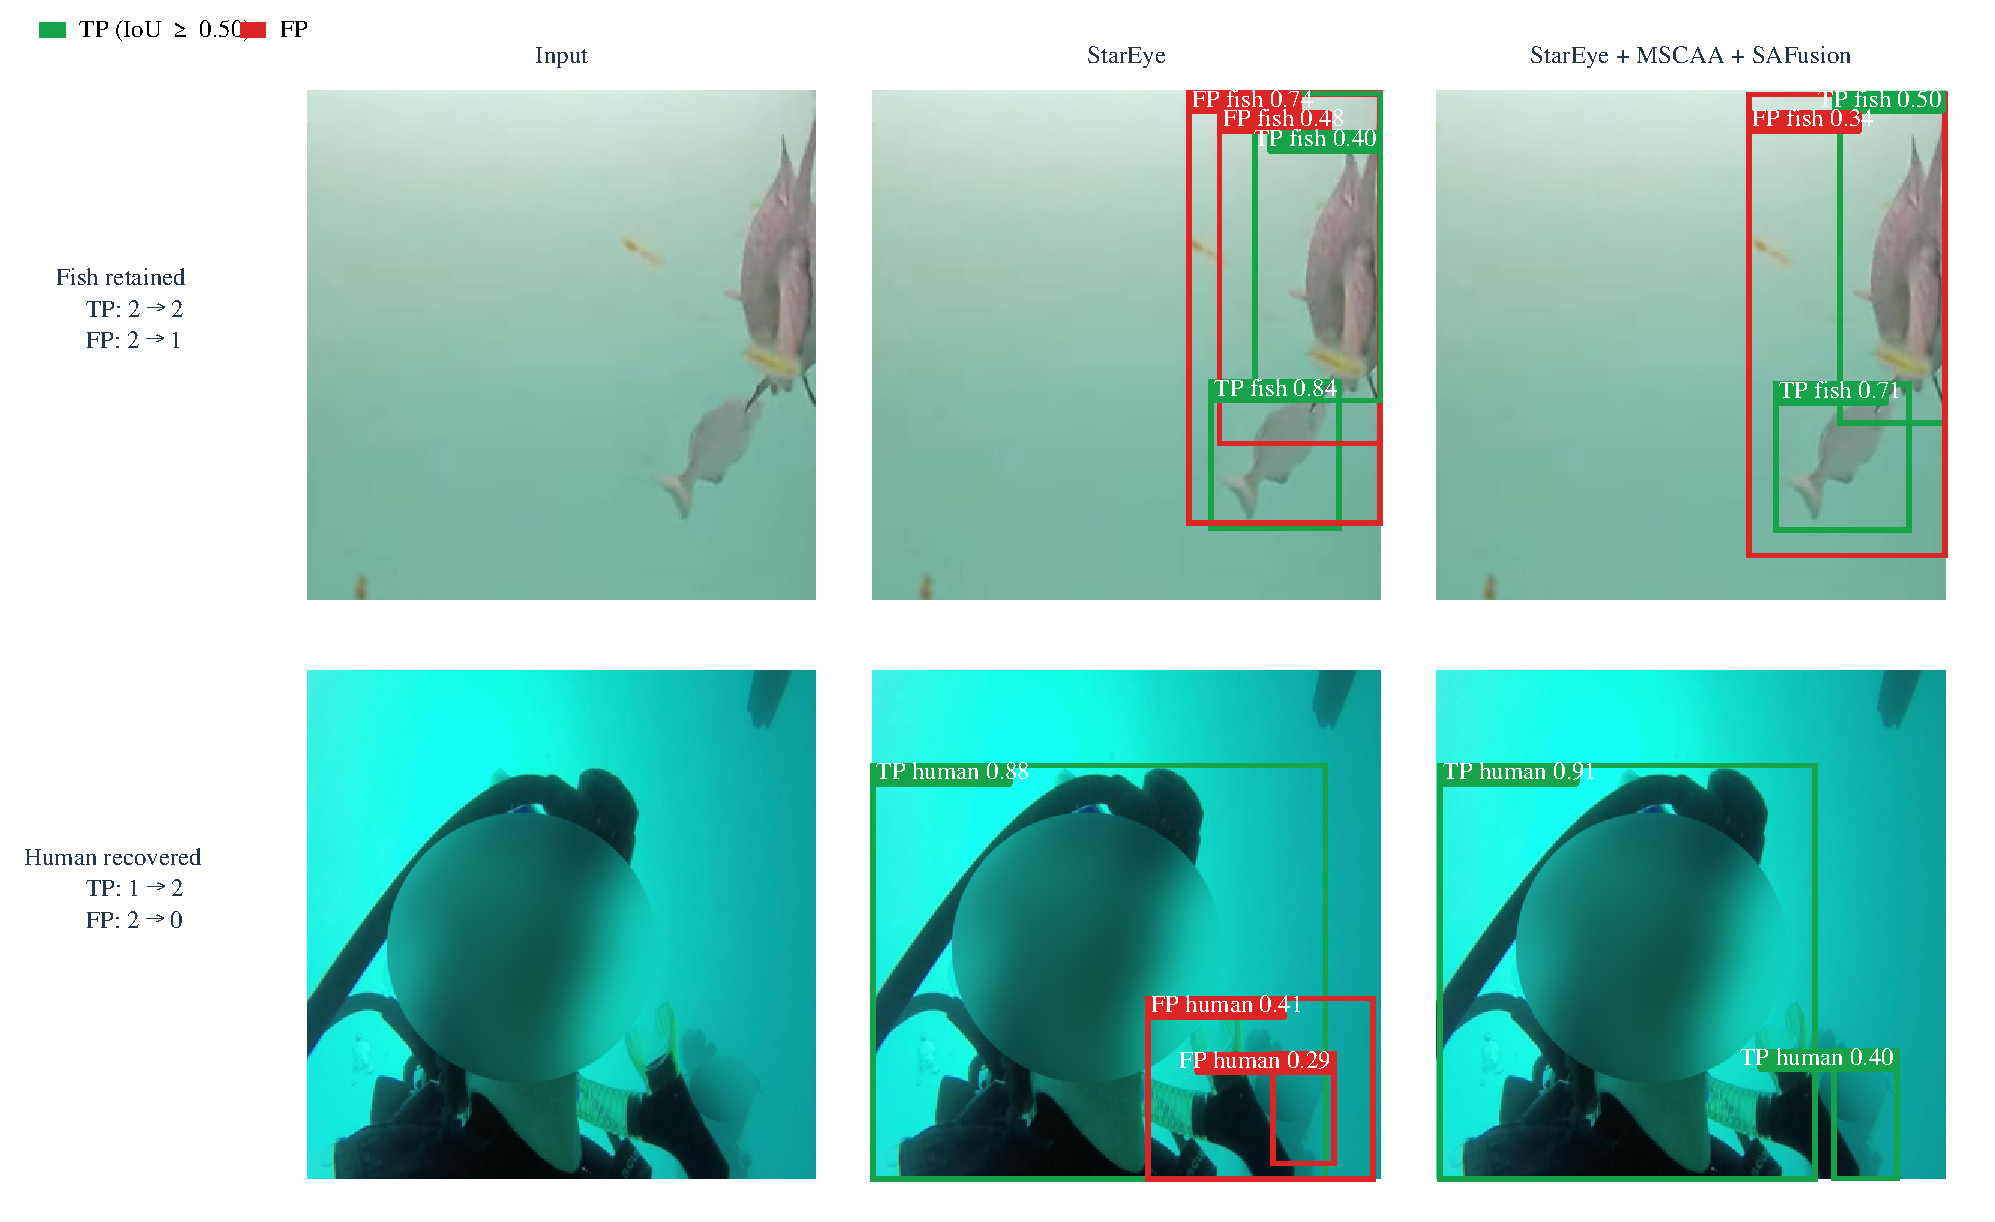
\includegraphics[width=0.92\textwidth]{joint_qualitative.pdf}
\caption{Seed-0 StarEye and joint-model predictions at confidence threshold
\(0.25\) and non-maximum suppression (NMS) IoU threshold \(0.70\).
Green/red boxes denote true/false positives (TPs/FPs); labels identify classes.
Class-consistent matching uses IoU \(0.50\).
The joint model retains both fish TPs and reduces FPs from two to one (top),
and recovers the missed human while removing two FPs (bottom).}
\label{fig:qualitative}
\end{figure*}

\subsection{Accuracy and Efficiency}
Table~\ref{tab:comparison} compares three-seed StarEye variants and gives two
pretrained generic detectors as capacity context. Only the final two rows share
architecture family, data, schedule, evaluator, and scratch initialization.

The proposed recalibration hierarchy improves mean validation AP from \(0.6143\) to \(0.6440\), yielding a \(2.97\)-point gain with only \(1.1\) additional reported GFLOPs. The improvement extends to both categories: human AP increases by \(2.28\) points and fish AP by \(3.67\) points. \(\mathrm{AP}_{50}\) also rises from \(0.9080\) to \(0.9446\).

% Keep Tables I and II side by side while retaining independent captions.
\begin{table*}[!t]
\centering
\begin{minipage}[t]{\columnwidth}
\vspace{0pt}
\centering
\caption{Detection Accuracy and Model Complexity}
\label{tab:comparison}
\setlength{\tabcolsep}{3.2pt}
\scriptsize
\begin{tabular}{lccccc}
\toprule
Method & Init. & \(\mathrm{AP}_{50}\) & AP & Human AP & Params. / FLOPs\\
\midrule
YOLOv8m & COCO & \(0.9450\) & \(0.6690\) & \(0.8200\) & \(25.8\,\mathrm{M}/78.7\,\mathrm{G}\)\\
RT-DETR-L~\cite{ref_rtdetr} & pretr. & \(0.5900\) & \(0.3560\) & \(0.5270\) & \(28.5\,\mathrm{M}/100.6\,\mathrm{G}\)\\
\midrule
StarEye & scratch & \(0.9080\) & \(0.6143\) & \(0.7764\) & \(3.07\,\mathrm{M}/24.6\,\mathrm{G}\)\\
Joint (ours) & scratch & \(0.9446\) & \(0.6440\) &
\(0.7992\) & \(3.62\,\mathrm{M}/25.7\,\mathrm{G}\)\\
\bottomrule
\end{tabular}
\par\vspace{1mm}
\parbox{\linewidth}{\centering\footnotesize Human AP: mean over IoU \(0.50\)--\(0.95\).
Joint: StarEye+MSCAA+SAFusion.
StarEye variants: three-seed means, same native evaluator.
Init. as listed.}
\end{minipage}\hfill
\begin{minipage}[t]{\columnwidth}
\vspace{0pt}
\centering
\caption{Three-Seed Mean Ablation of the Joint Calibration Design}
\label{tab:ablation}
\scriptsize
\resizebox{\linewidth}{!}{%
\begin{tabular}{cccccc}
\toprule
MSCAA & SAFusion & Overall AP & Overall \(\mathrm{AP}_{50}\) & Human AP & Fish AP\\
\midrule
 & & \(0.6143\) & \(0.9080\) & \(0.7764\) & \(0.4521\)\\
\checkmark & & \MSCAAAP & \MSCAAAPFifty & \MSCAAHumanAP & \MSCAAFishAP\\
 & \checkmark & \SAFusionAP & \SAFusionAPFifty &
  \SAFusionHumanAP & \SAFusionFishAP\\
\checkmark & \checkmark & \JointAP & \JointAPFifty &
  \JointHumanAP & \JointFishAP\\
\bottomrule
\end{tabular}
}
\par\vspace{1mm}
\parbox{\linewidth}{\centering\footnotesize Mean over seeds \(0\), \(42\), and \(123\);
per-seed values are retained in the evaluation record.}
\end{minipage}
\end{table*}

\subsection{Component Effects}
Table~\ref{tab:ablation} reveals complementary gain profiles for the two recalibration mechanisms. MSCAA provides a larger improvement for fish detection, increasing fish AP by \(2.49\) points, whereas SAFusion yields a larger improvement for human detection, increasing human AP by \(1.68\) points. The joint configuration achieves the highest three-seed mean for all four reported metrics among the four configurations. In overall AP, it exceeds MSCAA alone by \(1.34\) points and SAFusion alone by \(1.95\) points, producing a total gain of \(2.97\) points over the baseline. These results support the benefit of coordinating cross-source channel recalibration with dual-extent spatial refinement.

\subsection{Complexity and Factorial Interaction}
Accuracy gains come from recalibrating neck representations, rather than expanding backbone capacity or adding detection scales.

For a SAFusion input with \(C\) channels, its two projections contain \(2Cr\)
weights, where \(r=\max(\lfloor C/8\rfloor,8)\). The four gates add \(78{,}080\)
weights; the remaining increase comes from the MSCAA strip paths and fusion
projections. The complete design adds \(0.55\) million parameters and
\(1.1\) GFLOPs to StarEye, corresponding to increases of
\(17.9\%\) and \(4.5\%\), respectively. This targeted neck
modification improves overall AP by \(2.97\) percentage points
while preserving the original three-scale detection structure.

Let \(A_{00}\), \(A_{10}\), \(A_{01}\), and \(A_{11}\) denote the three-seed mean overall AP values of the
baseline, MSCAA-only, SAFusion-only, and joint configurations. Their factorial
interaction is
\begin{equation}
 \Delta_{\mathrm{int}}=A_{11}-A_{10}-A_{01}+A_{00}=\JointInteraction.
 \label{eq:interaction}
\end{equation}
The interaction of \(+0.0032\) means the joint gain in mean overall AP exceeds
the sum of the isolated gains by \(0.32\) percentage points. Together with its
advantage over either module alone, this descriptive comparison supports
empirical complementarity under the evaluated protocol.

\subsection{Qualitative Analysis}
Under identical inference settings, Fig.~\ref{fig:qualitative} shows that the
joint model preserves both true-positive fish detections while reducing false
positives from two to one, and recovers the missed human while removing two
false positives. These examples illustrate improved target retention and
reduced spurious responses, complementing the aggregate results in
Table~\ref{tab:ablation}.

\section{Conclusion}
This letter presents a hierarchical pyramid recalibration design
coordinating cross-source channel weighting with dual-extent spatial
refinement for lightweight underwater object detection. SAFusion at
cross-level fusion junctions and MSCAA within subsequent C2f-Star blocks
form an ordered fusion-to-refinement hierarchy, preserving the original
backbone and detection scales. On the evaluated two-class dataset,
the joint model improves three-seed mean validation AP by \(2.97\)
percentage points with \(4.5\%\) more FLOPs. Factorial ablation demonstrates
complementary contributions and higher mean AP than either module alone.
These results support neck-level recalibration for lightweight underwater
detection, with potential applications in robotic visual perception.


\bibliographystyle{IEEEtran}
\bibliography{references}

\end{document}
